\begin{figure}[H]
	\centering
	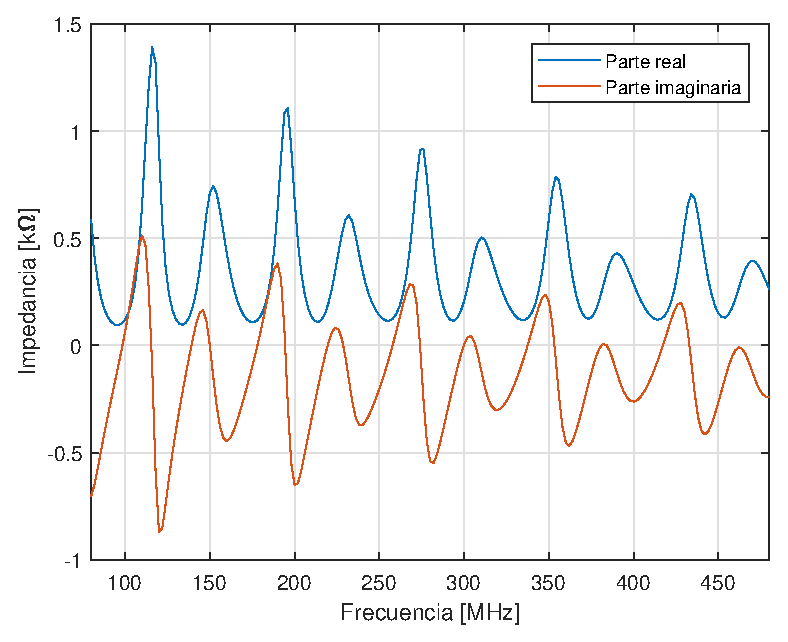
\includegraphics{imagenes/z_tierra.eps}
	\caption{Resistencia de radiación con plano a tierra perfecto.}
	\label{fig.z_radiacion}
\end{figure}


La impedancia de radiación para las frecuencias mínima y máxima analizadas resultan \label{ec.z_80_tierra} y \label{ec.z_480_tierra} respectivamente.

\begin{equation}
	\centering
	Z(\SI{80}{\mega\hertz}) = (571 - j \cdot 714) \Omega
	\label{ec.z_80_tierra}
\end{equation}

\begin{equation}
	\centering
	Z(\SI{480}{\mega\hertz}) = (257 -j \cdot 228) \Omega
	\label{ec.z_480_tierra}
\end{equation}		
